\subsection{Berechnung von Kugelvolumen und -dichte}
\begin{table}[h!]
\centering
\begin{tabular}{c | c | c}
	& groß & klein \\
	\hline
	& 15.802 & 15.651 \\
	& 15.796 & 15.652 \\
	& 15.804 & 15.650 \\
	\hline
	Mittelwert & \SI{15.801(2)}{} & \SI{15.651(1)}{}
\end{tabular}
\caption{Durchmesser $d$ der beiden Kugeln in \SI{e-3}{\metre}}
\label{fig:DatenKugel}
\end{table}
Aus den Durchmessern der zwei Glaskugeln (siehe Tabelle \ref{fig:DatenKugel}) ergeben sich die Volumina
\begin{align}
	V_\text{kl} &= \SI{2.0074(2)e-6}{\metre\cubed} \quad \text{und} \\
	V_\text{gr} &= \SI{2.0655(8)e-6}{\metre\cubed} \ .
\end{align}
Die kleinere Kugel wiegt
\[ m_\text{kl} = \SI{4.44e-3}{\kilo\gram} \]
und die größere
\[ m_\text{gr} = \SI{4.63e-3}{\kilo\gram} \ , \]
damit können auch die Dichten
\begin{align}
	\rho_\text{kl} &= \SI{2211.9(2)}{\kilo\gram\per\metre\cubed} \quad \text{und} \\
	\rho_\text{gr} &= \SI{2241.6(8)}{\kilo\gram\per\metre\cubed}
\end{align}
berechnet werden. Die Fehler ergeben sich hierbei durch die Gaußsche Fehlerfortpflanzung
\todo{Super! Mit Fehlerfortpflanzung :-)}
\begin{align}
	V(d) &= \frac{4}{3}\pi\left(\frac{d}{2}\right)^3: && \sigma_{V} = \left|\pdv{V}{d}\sigma_{d}\right| = 2\pi\left(\frac{d}{2}\right)^2\sigma_{d} \\
	\rho(d) &= \frac{m}{\frac{4}{3}\pi\left(\frac{d}{2}\right)^3}: && \sigma_{\rho} = \left|\pdv{\rho}{d}\sigma_{d}\right| = \frac{9m}{2\pi\left(\frac{d}{2}\right)^4}\sigma_{d} \ .
\end{align}
\clearpage

\subsection{Bestimmung der Apparatekonstante für die große Kugel}
\todo[color=red, inline]{Ich meine, Lena hätte gesagt, dass die Aperatkonstante überhaupt nicht mehr stimmt. Ich würde daher die Viskosität von Wasser bei 20 Grad nachschlagen  (\SI{1.005}{\milli\pascal\second}) und daraus die Konstante berechnen. Und die Viskosität gibt man standartmäßig in \si{\pascal\second} an. Abgesehen davon ist der Wert $\eta_{20}$ in der falschen Größenordnung. Als ich in gerade nachgerechnet habe, kam \SI{1.79}{\milli\pascal\second} heraus. }
\todo[color = green, inline]{Ah ja, das mit der Apparatekonstante stimmt. Das hatte ich vergessen. \\
Oh ja. Bei dem $\eta_{20}$ ist das milli verloren gegangen. \\
Die Einheit würde ich gerne beibehalten, weil Pascal keine SI-Einheit ist.}
\todo[color=green, inline]{Gegenargument: Newton ist auch keine SI-Einheit und ich würde trotzdem nicht \si{\kilo\gram\meter\per\second\squared} schreiben. Ich glaube Einheiten sind viel mehr eine Frage der Gewohnheit (solange sie sich aus SI-Einheiten zusammensetzen). Sehr wichtig ist mir das jetzt aber ehrlich gesagt nicht wirklich ;-) }
Die Messung der Fallzeit ergibt die Werte in Tabelle \ref{fig:DatenZeit}.
\todo[color=red]{Fallzeit in Sekunden}
\begin{table}[h!]
\centering
\begin{tabular}{c|c|c}
	& klein & groß \\
	\hline
	& 12.91 & 92.62 \\
	& 12.87 & 92.35 \\
	& 13.00 & 92.44 \\
	& 12.78 & 92.07 \\
	& 12.59 & 93.31 \\
	& 12.73 & 92.72 \\
	& 12.93 & 93.71 \\
	& 12.76 & 91.91 \\
	& 12.85 & 92.25 \\
	& 12.70 & 91.95 \\
	\hline
	Mittelwerte & \SI{12.81(4)}{} & \SI{92.5(2)}{}
\end{tabular}
\caption{Fallzeiten für ein \SI{0.10}{\metre} langes Rohr}
\label{fig:DatenZeit}
\end{table} \\
Mit der Viskosiät von Wasser bei \SI{20}{\celsius} bzw. \SI{293.15}{\kelvin}\footnote[3]{W. Walcher: Praktikum der Physik, Teubner Studienbücher, 1985, Tabellen-Anhang 1.7}
\[ \eta_{20} = \SI{1.002e-3}{\kilo\gram\per\metre\per\second} \]
und der Dichte von Wasser bei derselben Temperatur\footnotemark[3]
\[ \rho_\text{W} = \SI{992.8}{\kilo\gram\per\metre\squared} \]
können durch Umstellen und Einsetzen in Formel \eqref{Visk} die Apparatekonstanten für die kleine
\begin{align}
	K_\text{kl} = \frac{\eta_{20}}{(\rho_\text{kl}-\rho_\text{W})t_\text{kl}} = \SI{6.41(2)e-8}{\metre\squared\per\second\squared}
\end{align}
und die große Kugel
\begin{align}
	K_\text{gr} = \SI{8.67(2)e-9}{\metre\squared\per\second\squared}
\end{align}
bestimmt werden.
Auch bei diesen Werten ergibt sich der Fehler durch die Gaußsche Fehlerfortpflanzung
\begin{align}
	K &= \frac{\eta}{(\rho-\rho_\text{W})t}: && \sigma_K = \sqrt{\left(\pdv{K}{\rho}\sigma_\rho\right)^2+\left(\pdv{K}{t}\sigma_t\right)^2} \\
	& && \quad\ = \sqrt{\left(\frac{\eta\sigma_\rho}{(\rho-\rho_\text{W})^2t}\right)^2+\left(\frac{\eta\sigma_t}{(\rho-\rho_\text{W})t^2}\right)^2} \ .
\end{align}
\clearpage

\subsection{Konstantenbestimmung der Andradeschen Gleichung}
Bei der Fallzeit-Messung mit ansteigender Wasser-Temperatur werden die Werte in Tabelle \ref{fig:DatenTemperatur} gemessen. Eingesetzt in Gleichung \eqref{Visk} kann so die Viskosität des Wassers in Abhängigkeit der Temperatur berechnet werden. Diese Werte finden sich in derselben Tabelle. Wieder berechnet sich der Fehler der Viskosität nach Gauß ($K$ und $\rho$ sind dabei die Werte der großen Kugel):
\begin{align}
	\eta = K(\rho-\rho_\text{W})t: \qquad \sigma_{\eta} &= \sqrt{\left(\pdv{\eta}{K}\sigma_K\right)^2+\left(\pdv{\eta}{\rho}\sigma_{\rho}\right)^2 + \left(\pdv{\eta}{t}\sigma_{t}\right)^2} \\
	&= \sqrt{\left((\rho-\rho_\text{W})t\right)^2+\left(Kt\sigma_\rho\right)^2+\left(K(\rho-\rho_\text{W})t\sigma_t\right)^2} \ .
\end{align}
\begin{table}[h!]
\centering
\begin{tabular}{c|c|c|c|c}
	$T$ in \SI{}{\celsius} & \multicolumn{2}{ |c| }{Fallzeit in \si{\second}} & Mittelwert der Zeitmessungen & Viskosität $\eta(T)$ in \SI{e-3}{\metre\squared\per\second\squared} \\
	\hline
	20 & 92.25 & 91.95 & \SI{92(1)}{} & \SI{0.997(2)}{} \\
	28 & 83.25 & 78.72 & \SI{81(2)}{} & \SI{0.88(2)}{} \\
	31 & 74.78 & 73.89 & \SI{74.3(4)}{} & \SI{0.805(5)}{} \\
	35 & 67.97 & 76.66 & \SI{72(4)}{} & \SI{0.78(5)}{} \\
	40 & 62.19 & 62.64 & \SI{62.4(2)}{} & \SI{0.676(3)}{} \\
	45 & 57.69 & 56.56 & \SI{57.1(6)}{} & \SI{0.619(6)}{} \\
	51 & 51.68 & 51.78 & \SI{51.73(5)}{} & \SI{0.560(1)}{} \\
	55 & 48.21 & 49.78 & \SI{49.0(8)}{} & \SI{0.531(9)}{} \\
	60 & 45.63 & 45.06 & \SI{45.3(3)}{} & \SI{0.491(3)}{} \\
	65 & 42.47 & 41.50 & \SI{42.0(5)}{} & \SI{0.455(5)}{} \\
\end{tabular}
\caption{Fallzeiten der großen Kugel für ein \SI{0.10}{\metre} langes Rohr bei verschiedenen Wassertemperaturen und daraus berechnete Viskositäten}
\label{fig:DatenTemperatur}
\end{table}
 \\
Wird nun Gleichung \eqref{Andra} auf beiden Seiten logarithmiert, ergibt sich
\[ \ln\eta = \ln A + \frac{B}{T} \ , \]
mit
\[ X = \frac{1}{T} \quad \text{und} \quad Y = \ln\eta \]
kann so eine lineare Ausgleichsrechung mit den Werten in Tabelle \ref{fig:DatenRegression} durchgeführt werden.
\begin{table}[h!]
\centering
\begin{tabular}{c|c}
	$X=\frac{1}{T}$ in \SI{e-3}{\per\kelvin} & $Y=\ln\eta$ in \si{\ln\metre\squared\per\second\squared} \\
	\hline
	3.41 & -6.91 \\
	3.32 & -7.04 \\
	3.29 & -7.12 \\
	3.25 & -7.15 \\
	3.19 & -7.30 \\
	3.14 & -7.39 \\
	3.08 & -7.49 \\
	3.05 & -7.54 \\
	3.00 & -7.62 \\
	2.96 & -7.70
\end{tabular}
\caption{Werte, mit denen die Regression durchgeführt wird}
\label{fig:DatenRegression}
\end{table}

Mit Hilfe von Python errechnen sich die Konstanten
\begin{align}
	B &= \SI{1775(42)}{\kelvin\ln\metre\squared\per\second\squared} \\
	\ln A = \SI{-13.0(1)}{\ln\metre\squared\per\second\squared} \quad \Rightarrow \quad A &= \SI{2.4(3)e-6}{\metre\squared\per\second\squared} \ .
\end{align}
Die Gerade ist mit den Regressionswerten in Abbildung \ref{fig:Regression} zu sehen.
\begin{figure}[h!]
	\centering
	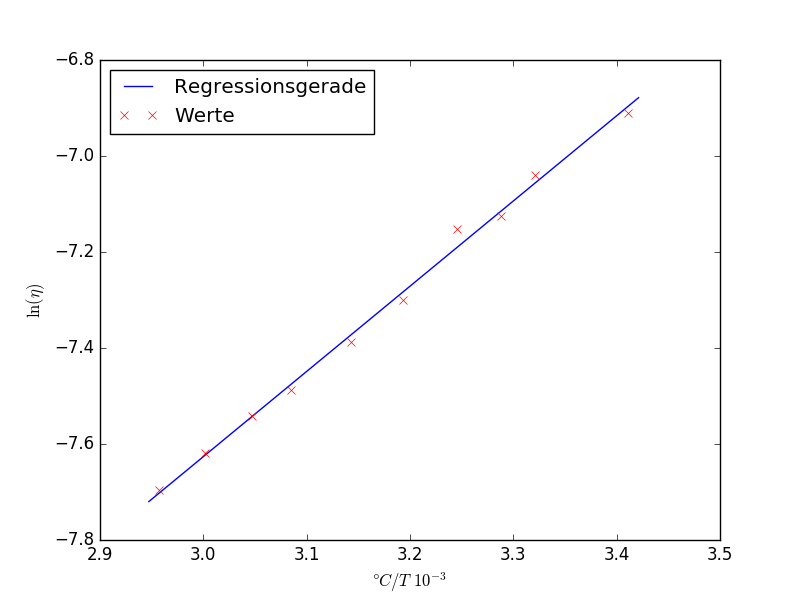
\includegraphics[width = 0.9\textwidth]{Regression.png}
	\caption{Regressiongerade mit Regressionswerten nach \eqref{Andra}}
	\label{fig:Regression}
\end{figure}
Die Andradesche Gleichung ist somit
\begin{align}
	\eta(T) = \SI{2.4e-6}{}\exp\left(\frac{1775}{T}\right) \ .
\end{align}
\clearpage

\subsection{Die Reynoldsche Zahl}
Zuletzt soll die Reynoldsche Zahl berechnet werden. Dafür wird benötigt
\begin{itemize}
	\item die Dichte von Wasser, sie ist eigentlich von der Temperatur abhängig, schwankt aber kaum im betrachteten Temperaturbereich, sodass weiterhin \[ \rho_\text{W}=\SI{992.8}{\kilo\gram\per\metre\cubed} \] angenommen wird;
	\item die Fließgeschwindigkeit des Wassers, welche gleich der Fallgeschwindigkeit
	\[ v = \frac{s}{t}, \quad s=\SI{0.10}{\metre} \] der Kugel ist;
	\item der Durchmesser des Zylinders, welcher gleich dem Durchmesser der Kugel \[ d = \SI{15.801e-3}{\metre} \] angenommen werden kann; und
	\item die temperaturabhängige Viskosität $\eta$.
\end{itemize}
Eingesetzt in \eqref{Reynolds} ergeben sich so die Werte in Tabelle \ref{fig:Reynolds}, die Fehler wiederum mit Gauß:
\begin{align}
	\text{RE} = \frac{\rho_\text{W} s d}{\eta t}: \qquad \sigma_{\text{RE}} &= \sqrt{\left(\pdv{\text{RE}}{t}\sigma_t\right)^2+\left(\pdv{\text{RE}}{d}\sigma_d\right)^2+\left(\pdv{\text{RE}}{\eta}\sigma_\eta\right)^2} \\
	&= \sqrt{\left(-\frac{\rho_\text{W}sd}{\eta t^2}\sigma_t\right)^2+\left(\frac{\rho_\text{W}s}{\eta t}\sigma_d\right)^2+\left(-\frac{\rho_\text{W}sd}{\eta^2 t}\sigma_\eta\right)^2} \ .
\end{align}
\begin{table}[h!]
\centering
\begin{tabular}{c|c}
	Temperatur in \si{\celsius} & $\text{RE}$ \\
	\hline
	20 & \SI{17.08(6)}{} \\
	28 & \SI{22.1(12)}{} \\
	31 & \SI{26.2(3)}{} \\
	35 & \SI{27.7(33)}{} \\
	40 & \SI{37.2(3)}{} \\
	45 & \SI{44.4(9)}{} \\
	51 & \SI{54.1(1)}{} \\
	55 & \SI{60.3(19)}{} \\
	60 & \SI{70.5(9)}{} \\
	65 & \SI{82.2(19)}{}
\end{tabular}
\caption{Errechnete Reynolds-Zahlen bei verschiedenen Temperaturen}
\label{fig:Reynolds}
\end{table}